\chapter{Design}
\label{chapter:design}

This chapter describes the current and proposed designs for managing vulnerability data, emphasizing scalability and efficient interaction between system components. Building on the multidimensional classification and remediation model outlined in chapter \ref{chapter:multidimensional-vulnerability-classification}, the proposed extension translates these concepts into a scalable and practical system design.

\section{Current Design}
\label{sec:current-design}

The current solution integrates data from the \ac{OSV} database into the internal system for vulnerability management. This process ensures efficient synchronization, processing, and storage of vulnerability advisories, aligning these advisories with components specified in the \ac{SBOM} to identify packages and components affected by vulnerabilities.

\begin{itemize}
    \item \textbf{Data Synchronization:} The system initiates synchronization by checking for the availability of the vulnerability data archive (\ac{OSV}) in a cloud-based storage system. This includes mechanisms to verify the freshness of the data (e.g., through metadata such as ETags) to avoid redundant processing. Only updated or newly added archives are retrieved and temporarily stored for processing. This process happens once a day.

    \item \textbf{Data Extraction and Processing:} Retrieved archives are decompressed, and individual advisories are parsed and processed. Each advisory is evaluated for updates since the last synchronization and is enriched with relevant details, such as identifiers, severity metrics, and associated packages. 
    \begin{itemize}
        \item \textbf{Change Detection:} Only advisories that have been modified since the previous synchronization are processed further.
        \item \textbf{Mapping and Enrichment:} Relevant details, including affected components, vulnerability types, and risk metrics (e.g., \ac{CVSS}), are extracted and structured for database integration.
    \end{itemize}

    \item \textbf{Component Alignment:} Processed advisories are matched against the components listed in the \ac{SBOM}. This step identifies specific packages and software elements within the \ac{SBOM} that are directly affected by vulnerabilities, enabling precise vulnerability reporting at the component level.

    \item \textbf{Database Update:} The structured advisories, enriched with mappings to specific components, are stored in the internal database. Synchronization metadata, such as timestamps and version identifiers, is updated to reflect the latest state of external data sources. When an \ac{API} request is triggered, the relevant data is sent to the frontend, ensuring the user interface always reflects the most recent vulnerability information.
\end{itemize}

\section{Extended Design}
\label{sec:extended-design}

The extended design centers on a streamlined approach to vulnerability information management. It integrates multiple data sources (e.g., vulnerability databases, scoring providers) and applies caching to reduce unnecessary network requests. Its purpose is to unify critical metrics (such as \ac{CVSS}, \ac{EPSS}) into a consolidated view, as described in the multi-dimensional classification model (see section \ref{sec:multi-dimensional-classification}), while also supporting role-specific actions based on the remediation model outlined in section \ref{sec:remediation_recommendation}.

\subsection{Backend Responsibilities}
\label{subsec:backend-responsibilities}

The backend is responsible for data retrieval, caching, and score computation, following the scoring algorithm described in section \ref{sec:algorithm-classifications}:
\begin{itemize}
    \item \textbf{Multi-Source Lookup:}  
    For each vulnerability, the system first queries the \ac{OSV} database to retrieve both the \ac{CVE} identifier and (if available) the \ac{CVSS} vector, leveraging \ac{OSV}'s integration of the entire \ac{GAD}.\footnote{\url{https://osv.dev/}} If no \ac{CVSS} vector is found there, the system sends a request to external sources (e.g., the \ac{NVD}), thereby minimizing the number of lookups. Similarly, the system always retrieves \ac{EPSS} data from the \texttt{first.org} database to ensure it remains up to date, as it is not included in the internal \ac{OSV} cache.
    \item \textbf{Caching and Time-Based Retrieval:}  
    The system initiates a daily update cycle by first attempting to retrieve \ac{CVSS} vectors from its local \ac{OSV} database. If unavailable, it sends individual requests to the \ac{NVD} for the missing \ac{CVSS} details, as batch queries for \ac{CVE} IDs are not supported.\footnote{\url{https://nvd.nist.gov/developers/vulnerabilities}} Simultaneously, batch requests are sent to the \texttt{first.org} database for \ac{EPSS} scores.
    After retrieving the new information, the cache is refreshed and any derived metrics (e.g., severity) are recalculated.
    \item \textbf{Role-Specific Recommendations:} Based on user input (e.g., developer or security advisor), the system determines a recommended course of action (see section \ref{sec:remediation_recommendation}). The backend solely stores the \ac{SSVC} recommendation, which might include immediate patching, hotfixes, or a scheduled approach, for later retrieval or review.
\end{itemize}

\subsection{Frontend Responsibilities}
\label{subsec:frontend-responsibilities}

The frontend is responsible for fetching data from the backend, displaying it to the user, and forwarding user inputs for storage. Key functionalities include:

\begin{itemize}
  \item \textbf{View Scores and Vectors:} A dedicated interface fetches data from the backend and displays \ac{CVE} identifiers, \ac{CVSS} vectors, \ac{CVSS} base scores, \ac{EPSS} values, overall severity, and missing data, as described in section \ref{subsec:ui-explaining-score}. Additionally, it is responsible for showing vulnerabilities ranked as described in section \ref{sec:rank-order-vulnerabilities}.
  \item \textbf{Perform Structured Assignments:} An interactive decision flow guides users (depending on their role) through a series of questions, ultimately generating a recommendation, as seen in the concept of section \ref{sec:remediation_recommendation}. 
  \item \textbf{Send Updates to the Backend:} Once the recommendation is finalized, it is transmitted to the backend for persistence.
\end{itemize}


\subsection{System Interaction Workflow}
\label{subsec:system-interaction}

This section outlines the mechanisms for updating, fetching, and caching vulnerability data. Figure~\ref{fig:data-fetch-flow} shows how the process begins with a scheduled update (e.g., at midnight) or an \ac{API} request from the frontend. In the latter case, if the vulnerability entity exists, the system returns it immediately; otherwise, a new record is created, and the creation or update process continues.

The backend checks if a \ac{CVE} is in the cache. If not, the workflow transitions to an \texttt{Error} state, returning a severity score of \textbf{10.1} (see section~\ref{subsec:handling-missing-data}), highlighted in pink on the frontend. Users can consult the \emph{Score Explanation} feature (see section~\ref{subsec:ui-explaining-score}) for guidance. If the \ac{CVE} exists, the system checks whether \ac{CVSS} data is cached. If unavailable, an external fetch is performed. The \ac{EPSS} metric is always retrieved externally to ensure it remains up to date, as it is not included in the cache.

Failure in either fetch leads to the \texttt{Error} state, while successful retrieval allows the system to compute an overall severity score (see section~\ref{sec:algorithm-classifications}) and store the final data. The process concludes by returning a fully updated record to the caller.

\begin{figure}[H]
\centering
\caption{The internal data-fetching, caching, and updating workflow for vulnerability data.}
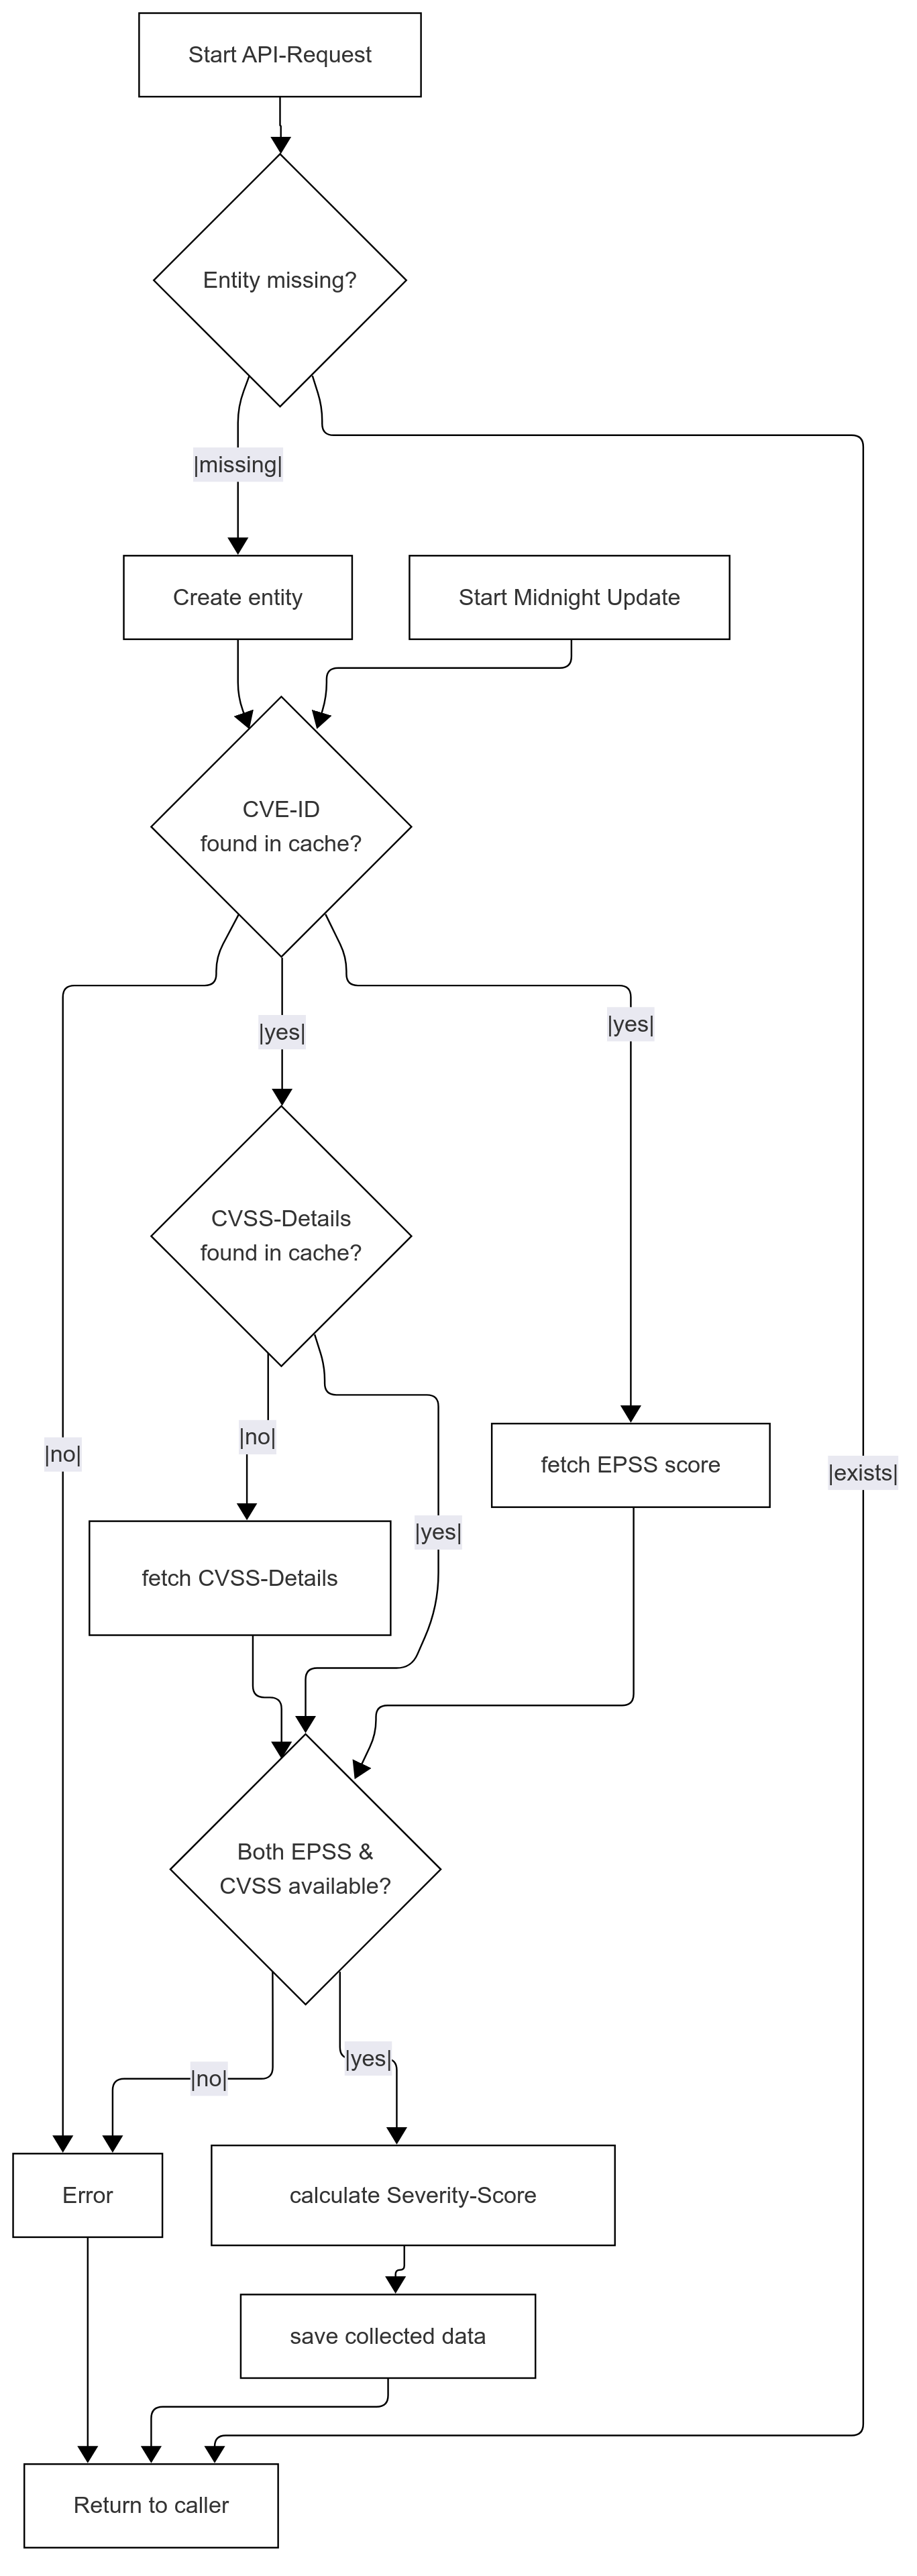
\includegraphics[width=1\textwidth,height=1\textheight,keepaspectratio]{resources/Data_Flow_Vulnerability_Data.png}
\label{fig:data-fetch-flow}
\end{figure}

\subsection{Rate Limits and Caching Benefits}
\label{subsec:rate-limits-caching}

In this design, \ac{CVE} data is exclusively retrieved from the local \ac{OSV} database, while \ac{CVSS} data is primarily obtained from the local \ac{OSV} database as well, querying the \ac{NVD} only if the required information is unavailable locally. Additionally, \ac{EPSS} data is fetched directly from \texttt{first.org}. External data sources impose rate limits to prevent misuse; for instance, the \ac{NVD} restricts queries to five requests per 30-second window without an \ac{API} key, and fifty with one.\footnote{\url{https://nvd.nist.gov/developers/start-here}} The \texttt{first.org} database enforces a threshold of 1,000 requests per hour without a token.\footnote{\url{https://api.first.org/\#Rate-Limit}} Since \ac{CVE} and most \ac{CVSS} data are retrieved locally from the \ac{OSV} database, no rate limits apply to these queries.

To cope with these constraints, the backend employs caching and batching to reduce repetitive lookups. Data retrieval occurs only when a record is missing or considered outdated, significantly minimizing external calls and reducing the risk of exceeding rate limits. During nightly updates, requests for \ac{EPSS} scores are processed in batches to further optimize efficiency. However, since the \ac{NVD} does not support batch queries for \ac{CVE} IDs,\footnote{\url{https://nvd.nist.gov/developers/vulnerabilities}} \ac{CVSS} data retrieval requires individual requests, making caching even more essential. Consequently, the system operates more reliably and gracefully handles errors by returning a severity score of \textbf{10.1} (see section~\ref{subsec:handling-missing-data}) whenever fetch errors occur. This condition is visually highlighted in pink on the frontend, prompting users to consult the score explanation interface (see section~\ref{subsec:ui-explaining-score}) to identify appropriate next steps for issue resolution.

\subsection{SSVC Process and Role-Specific Assignments}
\label{subsec:ssvc-process}

The \ac{SSVC} process involves tailoring vulnerability handling to each user's or team's specific context, following the stakeholder-specific prioritization framework described in section \ref{sec:algorithm-remediation}. This process is supported by the controller layer, which manages endpoints like the \ac{SSVC} recommendation endpoint. These endpoints facilitate the submission of role-specific decisions, which are then persisted and integrated with other metrics (e.g., \ac{CVSS}, \ac{EPSS}). Figure~\ref{fig:ssvc-interaction} illustrates this interaction.

\begin{figure}[H]
\centering
\resizebox{0.9\textwidth}{!}{%
\begin{tikzpicture}[>=stealth', node distance=2.5cm, auto, thick, font=\sffamily\small]

  \node[draw, rectangle, rounded corners, align=center, minimum width=3cm, minimum height=1cm] (frontend) {User Interface};
  \node[draw, rectangle, rounded corners, right=4.0cm of frontend, minimum width=3.3cm, align=center] (backendController) {Controller Layer};
  \node[draw, rectangle, rounded corners, right=3.5cm of backendController, minimum width=3.3cm, align=center] (backendStorage) {Data Storage \\ \& Calculation};

  \draw[->] (frontend.east)
    to[out=0, in=180]
    node[above, yshift=0.2cm]{\scriptsize Finalize Role-Based Decision}
    (backendController.west);

  \draw[->] (backendController.east)
    to[out=0, in=180]
    node[above, yshift=0.2cm]{\scriptsize Persist and Merge Data}
    (backendStorage.west);

  \draw[->] (backendStorage.south west)
    to[out=230, in=-50]
    node[below, yshift=-0.2cm]{\scriptsize Return Updated Metrics}
    (backendController.south east);

  \draw[->] (backendController.south west)
    to[out=230, in=-50]
    node[below, yshift=-0.2cm]{\scriptsize Updated Values (CVSS, EPSS, etc.)}
    (frontend.south east);

\end{tikzpicture}
}
\caption{High-level interaction in the \ac{SSVC} process.}
\label{fig:ssvc-interaction}
\end{figure}

\section{Conclusion}
\label{sec:design-conclusion}
The outlined design consolidates key vulnerability metrics and merges them with role-based inputs to yield tailored recommendations. By systematically checking internal data first and fetching new information only when required, it minimizes redundant requests while maintaining data accuracy. Frontend interactions are kept straightforward through specialized dialogs and status views, ensuring users can easily view or update vulnerability details. This approach offers a strong foundation for integrating further data sources and scaling to large application ecosystems.